\documentclass{beamer}

\usepackage[brazil]{babel}
\usepackage[utf8]{inputenc}
\usepackage{caption}
\usepackage{float}
\usepackage{listings}
\usetheme{Marburg}
\usecolortheme{beaver}
\setbeamertemplate{footline}[frame number]
\setbeamertemplate{caption}[numbered]
\setbeamertemplate{items}[ball]
\captionsetup{font=scriptsize,labelfont=scriptsize}
\title{Paradigmas de Programação da linguagem LUA}
\subtitle{Projeto Integrador VI}
\author{Mário Sergio e Pedro Martins}
\date{\today}

\begin{document}
\frame{\titlepage}


\begin{frame}[fragile]
	\begin{itemize}
	\frametitle{Paradigmas de Programação da linguagem LUA}
		\item Este projeto acadêmico se refere ao desenvolvimento de um estudo e pesquisa, relativo aos paradigmas e conceitos da linguagem de programação Lua.
			\begin{figure}[H]
			\centering
			
\includegraphics[width=0.3\linewidth]{imagens/logo}
			\caption{Logo - Lua Org}
			\end{figure}
	\end{itemize}
\end{frame}

\section{Roteiro}
\begin{frame}[fragile]
	\frametitle{Roteiro}
	\begin{itemize}
		\item Objetivos
		\item Motivações
		\item História da Linguagem
		\item Ánálise Léxica e Sintática
		\item Semântica das variáveis
		\item 
		\item 
		\item 
		\item Considerações Finais
	\end{itemize}
\end{frame}

\section{Introdução}
\subsection{Objetivos}
\begin{frame}[fragile]
	\frametitle{Introdução}
	{\bf Objetivos}\vspace{0.4cm}
	\begin{itemize}
		\item<1-> O objetivo do principal do projeto é aplicar os conhecimentos obtidos na disciplina de paradigmas de linguagem de programação à linguagem LUA.
		\begin{itemize}
			\item[$\mathbb{*}$]<2-> Levantar os paradigmas de programação da linguagem;
			\item[$\mathbb{*}$]<3-> Analisar Sintaxe e Semântica;
			\item[$\mathbb{*}$]<4-> Explicar e exemplificar o funcionamento de variáveis. Tipos, sua vinculação, verificação de tipo e escopo;
			\item[$\mathbb{*}$]<5-> Entender as vantagens, desvantagens e as áreas a qual LUA melhor se aplica;
			\item[$\mathbb{*}$]<6-> Criar códigos para exemplificar os conceitos apresentados. 
		\end{itemize}
	\end{itemize}
\end{frame}

\subsection{Motivações}
\begin{frame}[fragile]
	\frametitle{Introdução}
	{\bf Motivações}\vspace{0.4cm}
	\begin{itemize}
		\item <1-> Linguagem dinâmica, similar à python, ou seja, de fácil entendimento;
		\item <2-> Única linguagem criada fora do eixo de países desenvolvidos com relevância internacional;
		\item <3-> O nicho de aplicação de Lua é muito vasto;
		\item <4-> Leve, com apenas 20.000 linhas de código C que podem ser construídos em um intérprete executável 182K em um Linux;
	\end{itemize}
\end{frame}

\begin{frame}[fragile]
	\frametitle{Introdução}
	{\bf Motivações}\vspace{0.4cm}
	\begin{itemize}
		\item Portável, é utilizada em qualquer plataforma com um compilador C ANSI. Lua Pode ser usada em:
		\pause
		\item [$\mathbb{*}$] Microcontroladores; 
		\item [$\mathbb{*}$] Plataformas móveis;
		Consoles de jogos;
		\item [$\mathbb{*}$] Navegadores (traduzido para JavaScript);
		\item [$\mathbb{*}$] Aplicações de TV digital;
		\item [$\mathbb{*}$] Programas de manipulação de imagens.
	\end{itemize}
\end{frame}

\begin{frame}[fragile]
	\frametitle{Introdução}
	{\bf Exemplos de aplicações Lua}\vspace{0.4cm}
		\begin{figure}[H]
		\centering
		
\includegraphics[width=0.4\linewidth]{imagens/exemplo2}
		\caption{Jogos feitos em Lua}
		\end{figure}

		\begin{figure}[H]
			\centering
			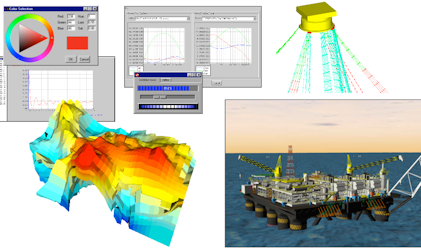
\includegraphics[height=2.5cm]{imagens/exemplo3}
			\label{figdroopy}
			\quad %espaco separador
			
\includegraphics[height=2.5cm]{imagens/exemplo1}
			\label{figsnoop}
			\caption{Aplicações Lua}
			\label{fig01}
		\end{figure}
\end{frame}


\section{História}
\begin{frame}[fragile]
\frametitle{História da Linguagem}
	{\bf Projeto Inicial}\vspace{0.2cm}
	\begin{itemize}
		\item <1-> A construção da linguagem veio de um projeto entre a PETROBRAS e a PUC-RIO, a fim de produzir um programa de interfaces gráficas para várias aplicações;
		\begin{figure}[H]
			\centering
			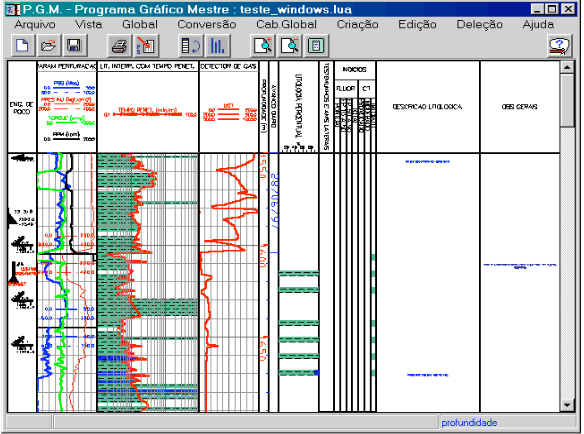
\includegraphics[width=0.2\linewidth]{imagens/imagem1}
			\caption{Programa Gráfico Mestre}
		\end{figure}
		\item <2-> Logo surgiu o DEL - Linguagem para Especificação de Diálogos;
		\item <3-> ‘SOL’ - Simple Object Language, uma linguagem para descrição de objetos,inspirada no bibTex.
		\begin{figure}[H]
			\centering
			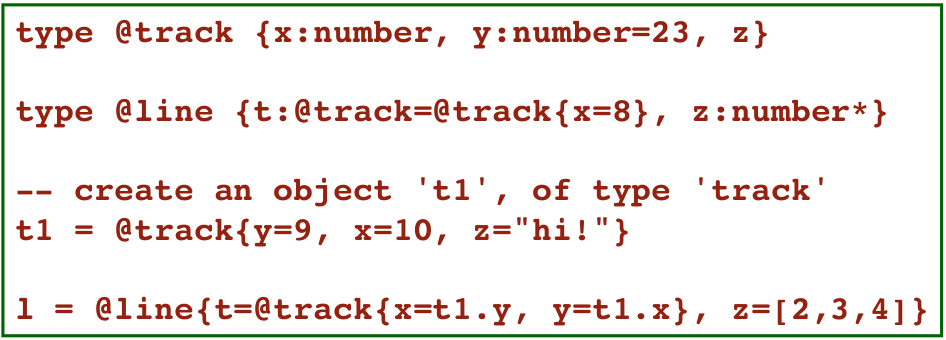
\includegraphics[width=0.3\linewidth]{imagens/imagem2}
			\caption{SOL}
		\end{figure}
	\end{itemize}
\end{frame}

\begin{frame}[fragile]
\frametitle{História da Linguagem}
	{\bf Esforço}\vspace{0.2cm}
	\begin{itemize}
		\item<1-> No entanto, DEL e SOL tinha várias limitações;
		\item<2-> As propostas de solução era formular uma nova linguagem de configuração genérica com as seguintes características:
		\begin{itemize}
			\item [$\mathbb{*}$]<3-> Facilmente acoplável;
			\item [$\mathbb{*}$]<4-> Portável
			\item [$\mathbb{*}$]<5-> Simples e de sintaxe fácil
		\end{itemize}
		\item<6-> Envolvidos: Roberto Ierusalimschy, Luiz Henrique de Figueiredo e Waldemar Celes;
	\end{itemize}
\end{frame}

\begin{frame}[fragile]
\frametitle{História da Linguagem}
	\begin{itemize}
		\item O resultado desse projeto foi dado o nome LUA, como um contraste da antiga SOL.
		\begin{figure}[H]
			\centering
			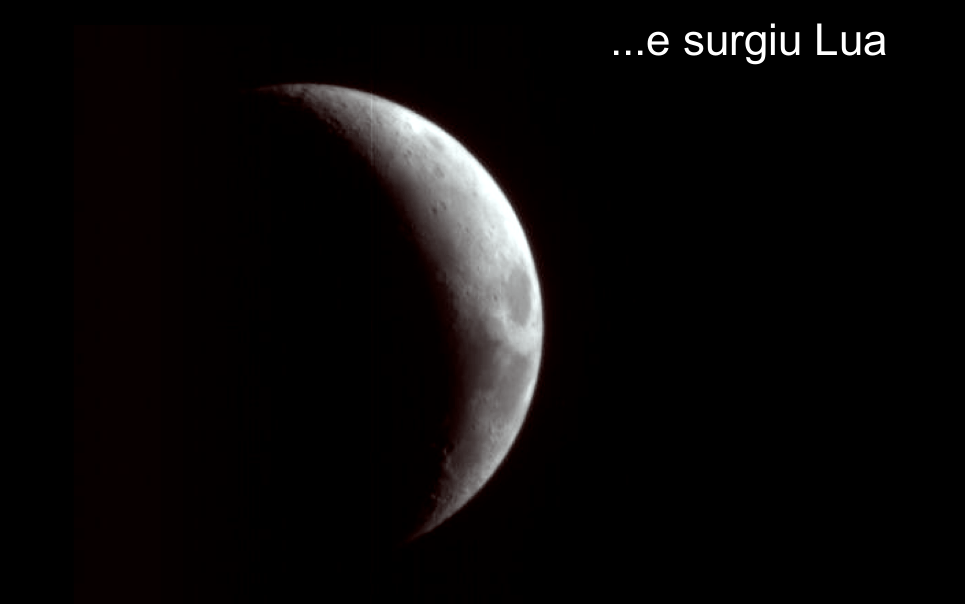
\includegraphics[width=1\linewidth]{imagens/lua}
		\end{figure}
	\end{itemize}
\end{frame}

\section{Ánálise Léxica e Sintática}
\subsection{Construções léxicas}
\begin{frame}[fragile]
\frametitle{Construções léxicas}
	\begin{itemize}
	\item<1-> Em Lua, os nomes podem ser qualquer cadeia de letras, dígitos, e sublinhados que não começam com um dígito; 
	\item<2-> Os identificadores são usados para nomear variáveis e campos de tabelas;
	\item<3-> Lua é uma linguagem que diferencia letras minúsculas de maiúsculas;
	\end{itemize}
\end{frame}

\subsection{Sintaxe}
\begin{frame}[fragile]
\frametitle{Sintaxe}
	\begin{itemize}
	\item Aqui está a sintaxe completa de Lua na notação BNF estendida. (Ela não descreve as precedências dos operadores). 
	\begin{figure}[H]
		\centering
		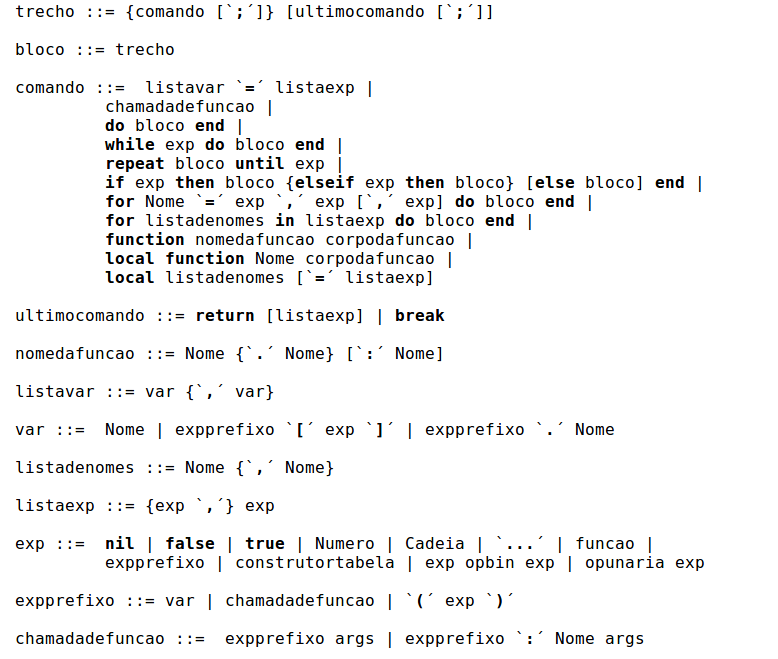
\includegraphics[width=0.9\linewidth]{imagens/sintaxe1}
	\end{figure}
	\end{itemize}
\end{frame}

\begin{frame}[fragile]
\frametitle{Sintaxe}
	\begin{figure}[H]
		\centering
		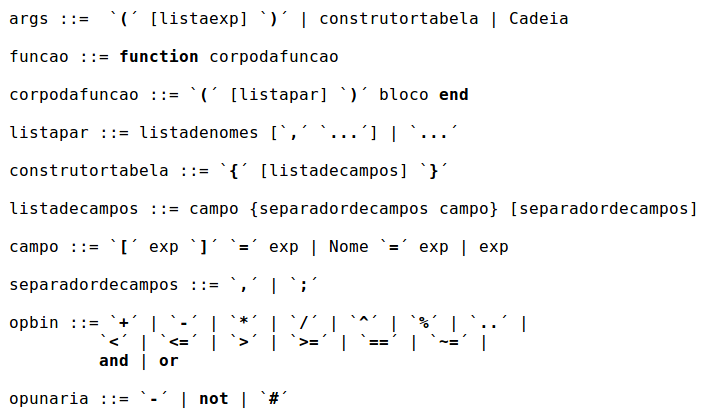
\includegraphics[width=1\linewidth]{imagens/sintaxe2}
	\end{figure}
\end{frame}

\section{Semântica das variáveis}
\subsection{Variáveis}
\begin{frame}[fragile]
\frametitle{Variáveis}
	\begin{itemize}
	\item <1-> Em Lua existem três tipos de variáveis, sendo elas as seguintes:
	\begin{itemize}
		\item [$\mathbb{*}$]<2-> Variáveis locais;
		\item [$\mathbb{*}$]<3-> Variáveis globais;
		\item [$\mathbb{*}$]<4-> Variáveis de tabelas.
	\end{itemize}
	\item <5-> A diferença entre variáveis locais e globais é o uso da palavra reservada ‘local’, antes do nome da variável.
	\begin{figure}[H]
	\centering
		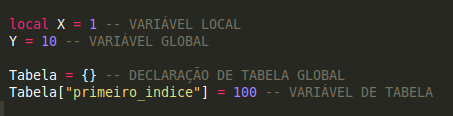
\includegraphics[width=0.7\linewidth]{imagens/variaveis}
	\end{figure}
	\end{itemize}
\end{frame}

\subsection{Vinculação}
\begin{frame}[fragile]
\frametitle{Vinculação}
	\begin{itemize}
	\item<1-> Lua é uma linguagem dinamicamente tipada; 
	\item<2-> A linguagem trabalha com vinculação dinâmica de tipos;
	\item<3-> Existem oito tipos de dados básicos em Lua:
	\begin{itemize}
		\item[$\mathbb{*}$]<4-> nil - boolean - number - string- thread;
		\item[$\mathbb{*}$]<5-> \textbf{function - userdata - table.}
	\end{itemize}
	\item<6-> O tempo de vida das variáveis é definido pelo fato de ela se global ou local;
	\end{itemize}
\end{frame}

\subsection{Verificação de Tipos}
\begin{frame}[fragile]
\frametitle{Verificação de Tipos}
	\begin{itemize}
	\item A verificação de tipos em Lua é feita em tempo de execução pelo interpretador Lua;
	\end{itemize}
	\begin{figure}[H]
			\centering
			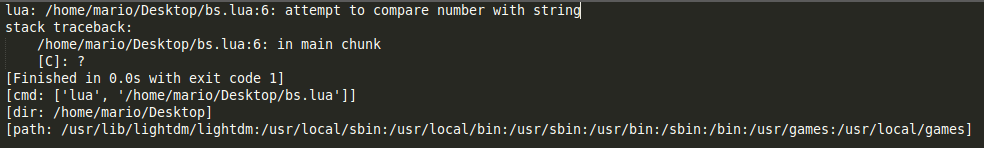
\includegraphics[width=0.3\linewidth]{imagens/verificacao_tipo}
			\caption{Trecho de código Lua}
	\end{figure}

	\begin{figure}[H]
			\centering
			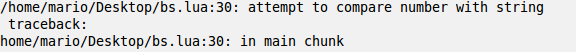
\includegraphics[width=1\linewidth]{imagens/verificacao_tipo2}
			\caption{Log de execução Lua}
	\end{figure}
\end{frame}

\subsection{Escopo}
\begin{frame}[fragile]
\frametitle{Escopo}
	\begin{itemize}
	\item<1-> Lua é uma linguagem com escopo léxico; 
	\item<2-> Baseia-se na sequência de chamadas de subprogramas;
	\item<3-> O escopo pode ser determinado em tempo de execução;
	\item<5-> Variáveis locais podem ser livremente acessadas por funções definidas dentro do seu escopo ou bloco;
	\begin{figure}[H]
			\centering
			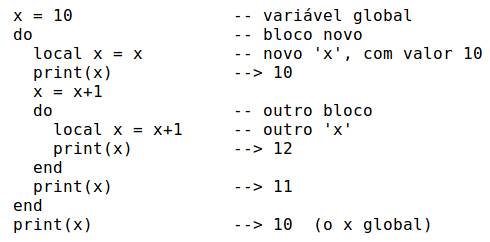
\includegraphics[width=0.6\linewidth]{imagens/imagem3}
			\caption{Trecho de código Lua}
		\end{figure}
	\end{itemize}
\end{frame}

\section{Conclusão}
\begin{frame}[fragile]
\frametitle{Conclusão}
	\begin{itemize}
	\item<1-> A iniciação do projeto foi a maior motivação para continuação do trabalho;
	\item<2-> O grupo compreendeu a complexidade de se aplicar os conceitos em um projeto de linguagem;\vspace{0.8cm}
	\item<3-> \textbf{Próximos Passos}
	\item[$\mathbb{*}$]<4-> Levantar os aspectos dos tipos de dados da linguagem Lua;
	\item[$\mathbb{*}$]<5-> Verificar a implementação e o comportamento dos subprogramas;
	\item[$\mathbb{*}$]<6-> Aprofundar no paradigma de `Orientação à tabelas' de Lua.
	\end{itemize}
\end{frame}

\end{document}